\documentclass[letterpaper]{article} % DO NOT CHANGE THIS
\usepackage{aaai2027}  % DO NOT CHANGE THIS
\usepackage[hyphens]{url}  % DO NOT CHANGE THIS
\usepackage{graphicx} % DO NOT CHANGE THIS
\urlstyle{rm} % DO NOT CHANGE THIS
\def\UrlFont{\rm}  % DO NOT CHANGE THIS
\usepackage{natbib}  % DO NOT CHANGE THIS AND DO NOT ADD ANY OPTIONS TO IT
\usepackage{caption} % DO NOT CHANGE THIS AND DO NOT ADD ANY OPTIONS TO IT
\frenchspacing  % DO NOT CHANGE THIS
\usepackage{amsmath}
\usepackage{booktabs}
\pdfinfo{
/TemplateVersion (2027.1)
}

\setcounter{secnumdepth}{1}

\title{Tools Help Per Question, Not on Average}
\author{Parsuram Pradhan}
\affiliations{
    parsuram.pradhan@yobytech.com
}

\begin{document}

\maketitle

\begin{abstract}
Agentic retrieval extends one-shot retrieval by letting a controller rewrite, search again, reorder passages, verify a draft, and stop. It remains difficult to decide when a step is worth its price, because answer quality treats a redundant search and a cheap reorder as the same action. We train a small policy over retrieve, rewrite, rerank, verify, and stop. The reward subtracts token dollars, retrieval dollars, latency, and a flat charge per action from answer quality, grounding, and calibration. Experiments on HotpotQA and Natural Questions, with BM25 and a frozen generator, train that policy with REINFORCE and select the checkpoint by greedy reward on held-out questions. Fixed recipes barely separate, while a per-question oracle over the same trajectories recovers a wide gap at nearly the one-shot price. Under the action charge the selected policy is one-shot retrieval; with every penalty removed it spends the step budget. When the retrieval score is usable, the learned policy rewrites a weak retrieval, searches again on a strong one, and leaves the verifier idle. A second training run does not repeat that controller. These results suggest that a priced tool helps on the question where it changes the answer, and that the controller spends it only when the objective makes the call worth its bill.
\end{abstract}

\section{Introduction}
A retrieval-augmented generator can search once and answer. An agentic loop can also rewrite the query, search again, reorder the passages, or check the draft before it stops. In a serving stack those steps do not share a price. A redundant search and a cheap reorder look the same to a controller that sees only exact match.

Learned search agents optimize answer quality, sometimes with a bonus for fewer turns \cite{jin2025searchr1,gandhi2026grasp}. Open-loop routers choose a depth from the question alone, before any passage is observed \cite{jeong2024adaptive}. Hand-written critics fire on thresholds \cite{asai2024selfrag,yan2024crag}. None of these tells a closed-loop policy when a priced tool is worth its bill.

This paper studies that decision in a small environment with a frozen generator, a frozen retriever, and an explicit reward. Figure~\ref{fig:pipeline} is the whole pipeline. The measurements support three claims.
\begin{itemize}
\item The flat action charge decides tool use. A full tool trajectory buys about 0.03 quality and pays about 0.10 in action charges. The selected policy is one-shot retrieval whenever that charge, or a large dollar weight, makes extra tools a losing bet, and it spends the step budget when every penalty is removed.
\item Tools help per question. Fixed recipes span 100 to 105 correct out of 300. An oracle that keeps the better logged answer on each question reaches 124, at nearly the one-shot price.
\item A 357-parameter policy can read retrieval strength and still miss the verifier. One threshold on the mean score reproduces 278 of 300 decisions at the second step. The verifier does not move exact match. A second training run does not repeat the controller.
\end{itemize}

\section{Related Work}
Retrieval-augmented generation conditions a generator on retrieved text \cite{lewis2020rag}. Agentic controllers interleave that retrieval with other tools. ReAct alternates reasoning traces and actions \cite{yao2023react}. The five systems in Table~\ref{tab:related} are the ones a reader will set this paper against. Each decides something about retrieval. None prices rewrite, rerank, and verify in dollars inside a closed loop.

\begin{table*}[t]
\centering
\small
\setlength{\tabcolsep}{4pt}
\begin{tabular}{lp{3.6cm}p{3.4cm}p{4.6cm}}
\toprule
Method & What it decides & What it prices & What we add \\
\midrule
Adaptive-RAG \cite{jeong2024adaptive} &
No retrieval, one retrieval, or multi-step retrieval, from the question alone &
Step count and relative time &
A second look after the passages arrive, with dollars and a per-action charge \\
Self-RAG \cite{asai2024selfrag} &
Whether to retrieve, and whether a segment is supported, as tokens in the generator &
Hand-set critique weights &
A frozen generator. Critique is one typed action with a measured cost \\
CRAG \cite{yan2024crag} &
Keep, discard, or mix the retrieved set. Discard triggers a web search &
An evaluator threshold &
Rewrite, rerank, and verify on a closed corpus \\
Search-R1 \cite{jin2025searchr1} &
When the language model itself emits a search during reasoning &
Answer correctness &
A small controller, so a change in exact match is a change in control \\
GRASP \cite{gandhi2026grasp} &
Semantic search, keyword search, or a paragraph read &
Answer quality, grounded reading, using both searches, and a turn count &
Rewrite, rerank, and verify, priced in dollars \\
\bottomrule
\end{tabular}
\caption{Published controllers this paper is positioned against. None is reimplemented on this stack. Adaptive-RAG is the row that could be: it is a classifier in front of no retrieval, one-shot retrieval, and a capped multi-step loop, all of which this environment already runs. That classifier is not trained here, so Adaptive-RAG is not a row in the results.}
\label{tab:related}
\end{table*}

Search-R1 trains the language model with an outcome reward to issue searches and reason over the results \cite{jin2025searchr1}. GRASP is the closest typed-action neighbor: a GRPO policy over semantic search, keyword search, and paragraph expansion, rewarded for answer quality, grounded reading, complementary search, and turn efficiency \cite{gandhi2026grasp}. GRASP does not price rewrite, rerank, or verification, and its efficiency term counts turns. We keep the generator fixed and ask a prior question: once those tools have a dollar cost, does a learned controller spend them only when they pay?

\section{Method}
Figure~\ref{fig:pipeline} is the protocol. An episode is one question. The controller picks one action at each step. The episode ends at stop, or when the step or budget cap forces a stop.

\begin{figure*}[t]
\centering
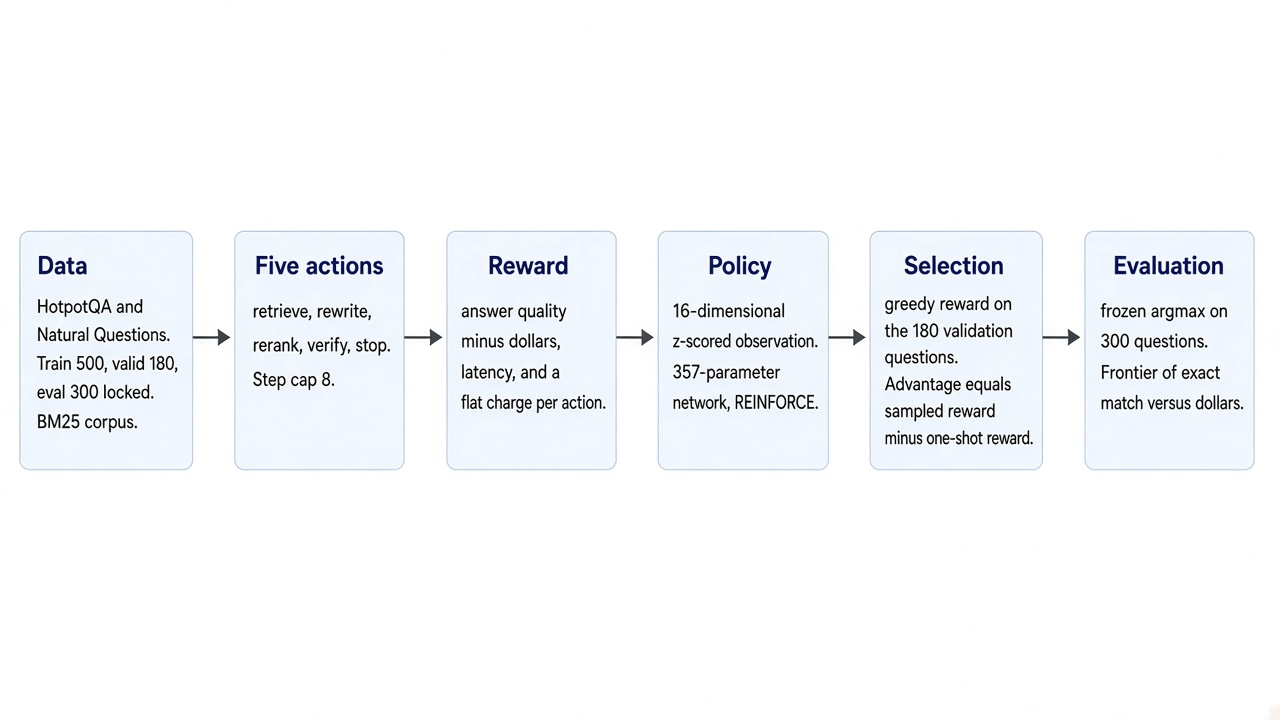
\includegraphics[width=\textwidth]{figures/pipeline.png}
\caption{The system. Data, the five-action environment, the reward, the policy and its training loop, and the locked evaluation that produces the frontier.}
\label{fig:pipeline}
\end{figure*}

\subsection{Actions, Retriever, and Generator}
The action set is retrieve, rewrite, rerank, verify, and stop. Retrieve runs BM25 \cite{robertson2009bm25} and appends the top five passages. Rewrite asks the generator for a new query. Rerank reorders the current pool by lexical overlap with the query. Verify runs a lexical natural-language-inference check of the current draft and returns support, neutral, or contradiction. Stop emits a short answer, or abstains. Yes/no questions must be answered yes or no. Caps are eight steps, three retrieves, two rewrites, two reranks, and two verifies. Illegal actions are masked: with no evidence the policy cannot rerank, verify, or stop.

The generator is Qwen2.5-3B-Instruct at temperature 0 \cite{qwen2024}. It reads the passages. The controller does not. The verifier is lexical, not a cross-encoder and not the generator judging itself. The price card meters local tokens at \$0.15 and \$0.60 per million input and output tokens, BM25 at \(5\times 10^{-5}\) dollars per call, and latency at \(10^{-3}\) dollars per second scaled by a latency weight. Absolute dollars are an instrumentation scale for a local model. Ratios are what the policy can learn.

\subsection{Observation, Training, and Selection}
The observation is 16 numbers. Four of them are retrieval scores: the mean of the top five, the top score, the gap between the top two, and the minimum of the top five. Each is a z-score against the training slice, clipped to \([-3, 3]\). The rest are the evidence count, remaining steps, remaining budget, verifier support and contradiction, the four tool counts, and a verify one-hot for support, contradiction, and neutral. There is no dataset indicator and no passage text. Before any retrieval the score channels are 0, the budget is full, and the vector does not contain the question. Every question therefore presents the same observation at step zero, and the first action cannot depend on which question is being asked. Adaptivity begins at the second step, after a retrieval has been observed.

The policy is a multilayer perceptron with one hidden layer of width 16, which is 357 parameters. Width above 32 is rejected. We train with REINFORCE \cite{williams1992reinforce} for 20 epochs. The return is the terminal reward below. The advantage on a training question is that question's sampled reward minus the reward of one-shot retrieval on the same question. The entropy bonus coefficient is 0.01, the optimizer is Adam, and the learning rate is 0.003. Training uses 500 questions, 300 from HotpotQA and 200 from Natural Questions. After each epoch we roll out the mode on a held-out 180, 110 HotpotQA and 70 Natural Questions. The checkpoint we report is the epoch with the highest greedy reward on that 180. It is chosen before the test set is opened. The test action is the mode of the masked softmax. We report seed 42, and a second training run at the same seed.

\subsection{Reward}
The terminal reward is
\begin{equation}
\begin{aligned}
R = {} & \alpha Q_{\mathrm{ans}} + \beta Q_{\mathrm{ground}} + \gamma Q_{\mathrm{cal}} \\
& - \lambda (C_{\mathrm{tok}} + C_{\mathrm{ret}}) - C_{\mathrm{lat}} \\
& - P_{\mathrm{hall}} - P_{\mathrm{act}} - P_{\mathrm{bud}} + B.
\end{aligned}
\label{eq:reward}
\end{equation}
\(Q_{\mathrm{ans}}\) is the average of exact match and token F1. \(Q_{\mathrm{ground}}\) mixes claim--evidence overlap with, on HotpotQA, recall of gold supporting titles. \(C_{\mathrm{tok}}\) and \(C_{\mathrm{ret}}\) are price-card dollars. \(C_{\mathrm{lat}}\) already includes the latency weight. \(P_{\mathrm{hall}}\) penalizes unsupported and contradicted claims. \(P_{\mathrm{bud}}\) is a unit penalty if a hard budget breaks. The unused-budget bonus \(B\) is granted only when \(Q_{\mathrm{ans}} \ge 0.5\). The action charge is \(P_{\mathrm{act}} = \rho \max(0, n-1)\) for \(n\) actions in the episode.

Default weights are \(\alpha{=}1\), \(\beta{=}0.4\), \(\gamma{=}0.15\), \(\lambda{=}2\), latency weight \(0.5\), hallucination weight \(0.5\), and \(\rho{=}0.02\). The learned runs below set \(\rho{=}0\) at \(\lambda{=}0\) and \(\lambda{=}20\), and \(\rho{=}0.02\) at \(\lambda{=}80\). A correct answer scores \(+0.3\) on the calibration term. Abstaining scores \(+0.6\) when the passage list is empty, the mean retrieval score is below 3, or verify returns contradiction, and \(-0.2\) otherwise. On this corpus the mean-score arm does not fire: raw BM25 means stay above 20, and means after the lexical reranker stay above 7. Empty evidence and a contradiction label still earn \(+0.6\). A wrong answer scores \(-0.4\) with evidence and \(-0.2\) without it.

\subsection{Data}
The test set is locked at 300 questions: 150 HotpotQA distractor items \cite{yang2018hotpotqa} and 150 Natural Questions items \cite{kwiatkowski2019nq}, disjoint from training and validation. The index holds HotpotQA contexts, unused HotpotQA distractors, and the DPR 100-word Wikipedia passages released with Natural Questions \cite{karpukhin2020dpr,gao2022tevatron}, including the passages needed by the 500 training and 180 validation questions, 83{,}120 passages in total. Gold text is a Wikipedia passage. BM25 recall at five on the evaluation questions is high on HotpotQA and well below one on Natural Questions, so a second retrieval can matter. Three frozen controllers define the corners of the cost plot: one-shot retrieval, a rule that reranks and verifies when the mean score is at least 3, and a max-tool policy that spends three retrieves, one rewrite, one rerank, and one verify.

\section{Results}

\subsection{The Charge Makes Extra Tools a Losing Bet}
Table~\ref{tab:frozen} is the frozen controllers. One-shot retrieval scores 100/300. Using every tool scores 105/300. The quality terms move by about 0.03: \(Q_{\mathrm{ans}}\) rises by 0.021, \(Q_{\mathrm{ground}}\) by 0.018, and \(Q_{\mathrm{cal}}\) by 0.009. The action charge rises from 0.02 to 0.12. Scaled dollars and latency together rise by about 0.002. A quality term of 0.03 against a charge of 0.10 is a reward loss of about 0.07, from 0.580 to 0.509. Of the penalty that separates the two trajectories, about 99 percent is \(\rho\) and about 1 percent is the price card. One extra retrieval costs roughly \(3\times 10^{-4}\) in the \(\lambda{=}2\) dollar term and 0.02 in \(\rho\), so the flat charge is about sixty times the measured dollar price of that call. The rule policy pays for a rerank and a verify on every question, lands between them on cost and reward, and does not improve exact match.

\begin{table}[t]
\centering
\setlength{\tabcolsep}{3pt}
\small
\begin{tabular}{lrrrr}
\toprule
Policy & Hotpot & NQ & Correct & \$ \\
\midrule
One-shot & 59/150 & 41/150 & 100/300 & \(1.72\times 10^{-4}\) \\
Rule & 56/150 & 41/150 & 97/300 & \(5.04\times 10^{-4}\) \\
Max tools & 61/150 & 44/150 & 105/300 & \(7.47\times 10^{-4}\) \\
\bottomrule
\end{tabular}
\caption{Frozen controllers. Hotpot is HotpotQA. One-shot retrieval has the highest reward (0.580). The max-tool policy has the highest exact match and the lowest reward (0.509). These three rows were scored before the training and validation passages entered the index. They are the corners of Figure~\ref{fig:frontier}, not rows of Table~\ref{tab:learned}.}
\label{tab:frozen}
\end{table}

The learner follows the arithmetic. With the action charge left on, including when the dollar and latency weights are zero, argmax evaluation is retrieve-then-stop on all 300 questions. Removing every penalty, so the return is \(Q_{\mathrm{ans}}\) alone, moves the same trainer off that mode: it spends the eight-step budget, three retrieves, two rewrites, and two verifies, and exact match rises from 100/300 to 102/300. At \(\lambda{=}80\), the extra max-tool dollars are about \(80 \times 5.8\times 10^{-4} \approx 0.046\), larger than the 0.03 quality those tools buy, and the action charge is also on. The selected policy is again retrieve-then-stop. The price card is not what pins the policy. The charge is, and at a high enough dollar weight the price card is enough on its own.

\subsection{A Flat Frontier, and the Gap Inside It}
Figure~\ref{fig:frontier} plots exact match against dollars for the frozen controllers, the selected learned checkpoints of the dollar sweep, and three oracles over trajectories logged in that sweep. The selected checkpoints sit on one-shot retrieval. The last epoch at \(\lambda{=}0\) is a six-step recipe, one retrieve and two rewrites and two verifies, at 104/300. The selection rule, fixed before the test set is opened, does not pick it: on the training questions that recipe scores lower than one-shot retrieval. Against one-shot retrieval the recipe repairs 6 HotpotQA answers and breaks 12, and repairs 18 Natural Questions answers and breaks 8.

\begin{figure*}[t]
\centering
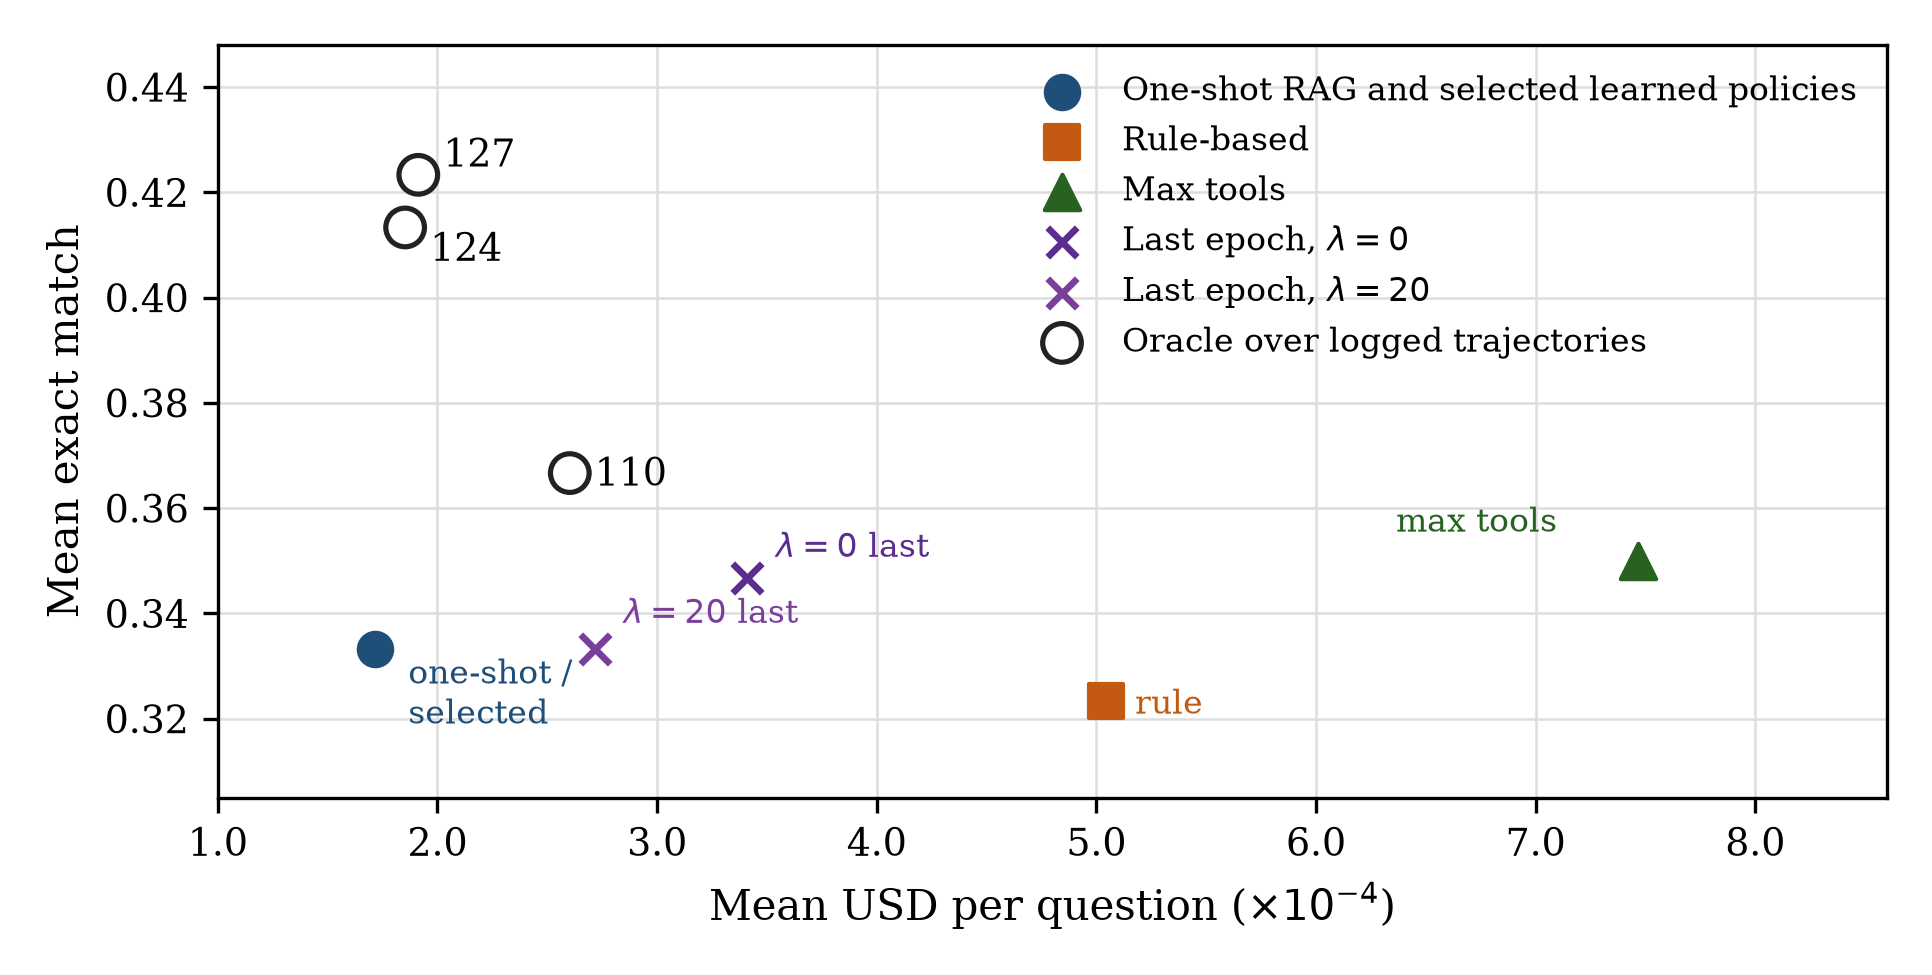
\includegraphics[width=0.92\textwidth]{figures/frontier.png}
\caption{Exact match against mean dollars per question for the frozen controllers and the dollar sweep. Squares are frozen controllers. Filled circles are selected learned checkpoints; they sit on one-shot retrieval. Crosses are last-epoch recipes the training reward did not select. Hollow circles are oracles over logged trajectories: 110 keeps one-shot retrieval on HotpotQA and the six-step recipe on Natural Questions; 124 keeps the better of those two answers on each question; 127 may also use the max-tool trajectory. Learned checkpoints from Table~\ref{tab:learned} are omitted: they were scored after the training passages joined the index.}
\label{fig:frontier}
\end{figure*}

An oracle that keeps the better of the two answers on each question scores 124/300 at \(1.85\times 10^{-4}\) dollars, close to the one-shot price, because it pays for the long trajectory only where the answer changes. Restricting the oracle to one-shot retrieval on HotpotQA and the six-step recipe on Natural Questions scores 110/300 at about a third of the max-tool bill. Allowing the max-tool trajectory as a third option scores 127/300. Single policies span 100 to 105 correct. The 24-answer gap from 100 to 124 is the room a controller has if it reads the question in front of it. A dataset bit would be enough for the jump to 110, and the observation does not contain one. The jump to 124 requires a per-question choice.

Table~\ref{tab:learned} is that controller under the protocol in Section 3, scored against one-shot retrieval on the same index. One-shot retrieval there is 100/300, HotpotQA 60/150 and Natural Questions 40/150, at \(1.72\times 10^{-4}\) dollars. The best learned checkpoint is 104/300. The gain over one-shot retrieval on this index is four answers, not the twenty-four the oracle shows on the earlier trajectories.

\begin{table*}[t]
\centering
\small
\setlength{\tabcolsep}{4pt}
\begin{tabular}{llrrrr}
\toprule
Run & Checkpoint & Correct & Sequences & Steps & \$ \\
\midrule
1 & \(\lambda{=}20\) & 103/300 & 16 & 7.49 & \(5.31\times 10^{-4}\) \\
1 & \(\lambda{=}0\) & 100/300 & 2 & 3.97 & \(3.11\times 10^{-4}\) \\
1 & \(\lambda{=}80\) & 100/300 & 1 & 2.00 & \(1.72\times 10^{-4}\) \\
2 & \(\lambda{=}0\) & 104/300 & 15 & 7.65 & \(5.37\times 10^{-4}\) \\
2 & \(\lambda{=}20\) & 104/300 & 6 & 5.89 & \(4.14\times 10^{-4}\) \\
2 & \(\lambda{=}80\) & 100/300 & 1 & 2.00 & \(1.72\times 10^{-4}\) \\
\bottomrule
\end{tabular}
\caption{Selected checkpoints of the 357-parameter policy. Both runs use seed 42. Sequences is the number of distinct action strings on the 300 questions. One-shot retrieval on this index scores 100/300 at \(1.72\times 10^{-4}\) dollars. \(\lambda{=}80\) matches it. These rows are not comparable to Table~\ref{tab:frozen}.}
\label{tab:learned}
\end{table*}

\subsection{Retrieval Strength, and an Idle Verifier}
On the first run, the selected \(\lambda{=}20\) policy emits 16 action sequences and scores 103/300 (HotpotQA 59/150, Natural Questions 44/150). Against one-shot retrieval on the same index that is \(+8\) answers and \(-5\). The branch is readable. At the second step, the first step that can see a retrieval, a threshold on the mean score at 45.7 reproduces 278 of 300 decisions. Weaker retrieval is rewritten. Stronger retrieval is searched again. The selected \(\lambda{=}0\) policy scores 100/300 with two sequences. It verifies about twice per question, changes 0 of 300 predictions relative to one-shot retrieval, and costs \(3.11\times 10^{-4}\) dollars against \(1.72\times 10^{-4}\).

The verifier is informative and unused as a reason to change the answer. A contradiction label occurs on 14 of 300 questions. Exact match on all 14 matches one-shot retrieval, so the label does not move the score: the bound on what this verifier changes is 0 answers inside those 14 questions, not a gain on the other 286, where the label never fires as a contradiction. On the branching run, a new retrieval follows a contradiction on 8 steps and stop follows it on 6. Support is followed by a new retrieval on 124 of 452 steps. The label and the retrieval score move together, so the split is an association with the feature the threshold already explains. On the second run the selected \(\lambda{=}0\) policy verifies twice per question, a contradiction is followed by a new retrieval or rewrite on 0 of 28 steps, and the 300 answers match the \(\lambda{=}20\) checkpoint exactly. The verifies cost \(5.37\times 10^{-4}\) dollars against \(4.14\times 10^{-4}\) for the same answers.

\subsection{A Second Run Does Not Repeat the Controller}
The second run, same protocol and same seed, ties the selected \(\lambda{=}0\) and \(\lambda{=}20\) checkpoints at 104/300, HotpotQA 60/150 and Natural Questions 44/150, with identical predictions. \(\lambda{=}20\) is one six-step recipe on 270 of 300 questions, and that recipe holds the whole gain over one-shot retrieval (\(+9\) and \(-5\), union 109/300) at \(4.14\times 10^{-4}\) dollars. \(\lambda{=}0\) uses 15 sequences. Best exact match moves from 103 to 104, one answer. What repeats is \(\lambda{=}80\): retrieve-then-stop on every greedy epoch, and the same 300 predictions as the first run. What does not repeat is the 16-sequence controller. Two runs at one seed cannot separate a four-answer gap from the draw. They can separate a controller that appears once from a controller that appears twice.

\subsection{Diagnostics}
An earlier observation passed the mean BM25 score through \(\tanh(\mathrm{score}/5)\). Top-1 scores on this corpus run from about 26 to 122, so that feature was 1.0 on all 300 questions and the policy could not branch on it. With validation selection and that observation, the \(\lambda{=}0\) checkpoint was one six-step recipe at 103/300, and the \(\lambda{=}20\) and \(\lambda{=}80\) checkpoints were one-shot retrieval. The recipe was one string on every question. Standardizing the score is what makes the branch in Table~\ref{tab:learned} expressible. The earlier numbers are the reason the branch had to be checked, not a second result.

\section{Limitations}
The policy never reads passage text. This is a study of the reward and of credit assignment in a 357-parameter controller, not of GRPO fine-tuning of the generator. Both learned runs in Table~\ref{tab:learned} use seed 42. A second run at the same seed is not a seed sweep. The planned final run, if the compute budget allows, is three fresh trainings at seeds 42, 43, and 44, reported as the three values or as a min--max range. Seeds multiply training only. The frozen controllers are deterministic at temperature zero.

Table~\ref{tab:frozen} and Figure~\ref{fig:frontier} were scored before the training and validation passages entered the index. Table~\ref{tab:learned} was scored after. The frozen rule and max-tool policies, and the ceilings 110, 124, and 127, have not been rebuilt on the later index, so they are not placed in Table~\ref{tab:learned}. The first action is identical across questions in every run, because the observation at step zero does not contain the question. The verifier and the reranker are lexical. The price card's absolute level is a local-model scale; the finding is the ratio of \(\rho\) to that scale. A neural verifier, a dense retriever, or a generator-sized policy could change the 0.03 quality gap, which would move the break-even dollar weight. We did not run that comparison. Adaptive-RAG, Self-RAG, CRAG, Search-R1, and GRASP remain Table~\ref{tab:related}, not rows in the results.

\section{Conclusion}
Tools help per question. Fixed recipes span 100 to 105 correct out of 300, and an oracle over trajectories already in hand answers 124 at nearly the one-shot price, because it pays for the long trajectory only where the answer changes.

The flat action charge explains the average. A full tool trajectory buys about five exact-match answers and pays about 0.10 in action charges, against a measured dollar and latency gap of about 0.002. The selected policy is one-shot retrieval when that charge, or \(\lambda{=}80\), makes extra tools a losing bet, and the same trainer spends the step budget when every penalty is removed.

A score the policy can actually read changes the controller and not the gap. The selected policy then branches on retrieval strength, leaves the verifier idle, and reaches 103 or 104 correct. A second training run does not repeat the controller. Closing the gap from 100 to 124 requires a branch that survives another run, trained against an objective in which a useful tool call is cheaper than the answer it buys.

\section*{Ethical Statement}
Pricing a tool has a use and a risk, and this paper measures both. The use is that a system can decline a search that does not buy an answer. The risk is who pays for that decline. Fixed recipes span 100 to 105 correct out of 300. A per-question choice among the same trajectories reaches 124, at nearly the one-shot price. The 24 answers in that gap are the ones a cost term refuses to pay for. A user who receives the cheap answer is not told that a second search would have changed it.

A cost term can also be satisfied by refusing to answer. Calibration pays \(+0.6\) for abstention when the passage list is empty, the mean retrieval score is below 3, or verify returns contradiction, and it penalizes a confident wrong answer more than an answer with no evidence. On this corpus the mean-score arm does not fire: raw BM25 means stay above 20, and reranked means stay above 7. The guard that was written for a weak retrieval never applies. The checkpoints selected under the default action charge do not abstain their way out of errors either. They match one-shot retrieval, including its errors, and they never call the verifier. That ships an unsupported answer at the price of a single search.

The verifier does find trouble. A contradiction label occurs on 14 of 300 questions, and exact match on all 14 still matches one-shot retrieval. On the second training run a contradiction is followed by a new retrieval or rewrite on 0 of 28 steps. A deployed copy of this controller would present a contradicted draft as the answer. The controller never reads passage text, so it also cannot tell that a passage is about a person, is off the question, or should not be shown. HotpotQA and Natural Questions are English Wikipedia questions, and the errors are not spread evenly across them: the six-step recipe that the training reward does not select repairs Natural Questions and breaks HotpotQA. A policy that copies one-shot retrieval copies that pattern.

The dollar amounts are an instrumentation scale for a local 3B model, not a bill a person pays. Treating them as a production budget would understate a hosted generator and could be cited as a reason to skip verification. The questions and passages are public benchmarks. No human subjects were involved. We report these failures and do not present these checkpoints as a serving policy.

\bibliography{references}

\end{document}
